% ********** Rozdział 4 **********
\chapter{Warstwa użytkowa projektu}
\section{Menu główne}


Jest to główne menu aplikacji, które użytkownik widzi po uruchomieniu programu. Zapewnia dostęp do podstawowych funkcji systemu, takich jak dokonywanie zakupów, logowanie się na konto admina oraz wyjście z aplikacji. Użytkownik może poruszać się po opcjach menu za pomocą odpowiednich znaków.



\begin{figure}[H] 
    \centering
    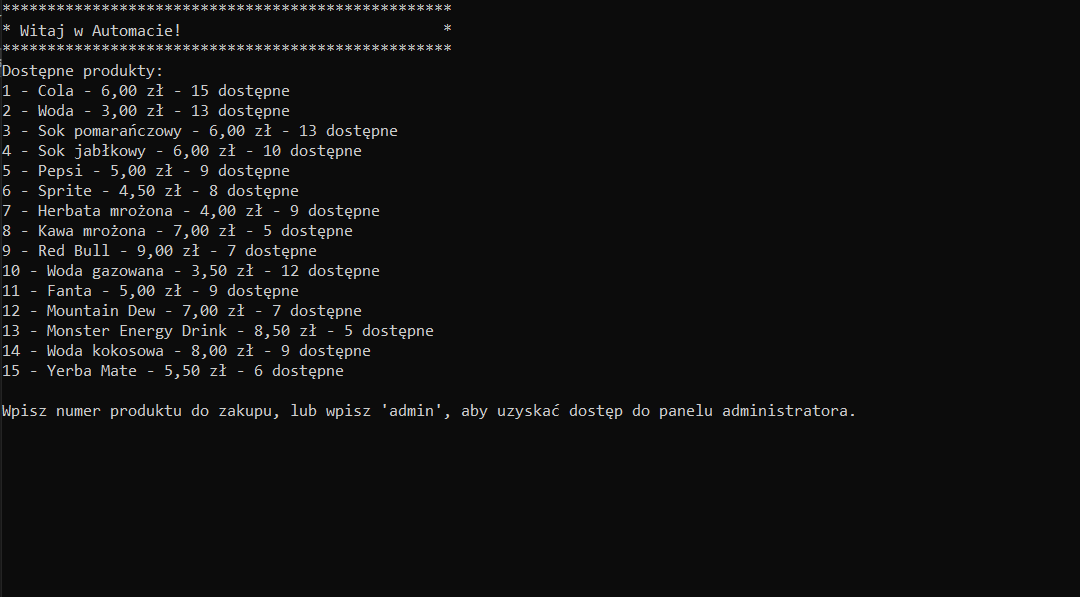
\includegraphics[width=0.8\textwidth]{grafiki/menu_glowne.PNG}
    \caption{\footnotesize Menu główne}	
\end{figure}

\newpage

\begin{figure}[H] 
    \centering
    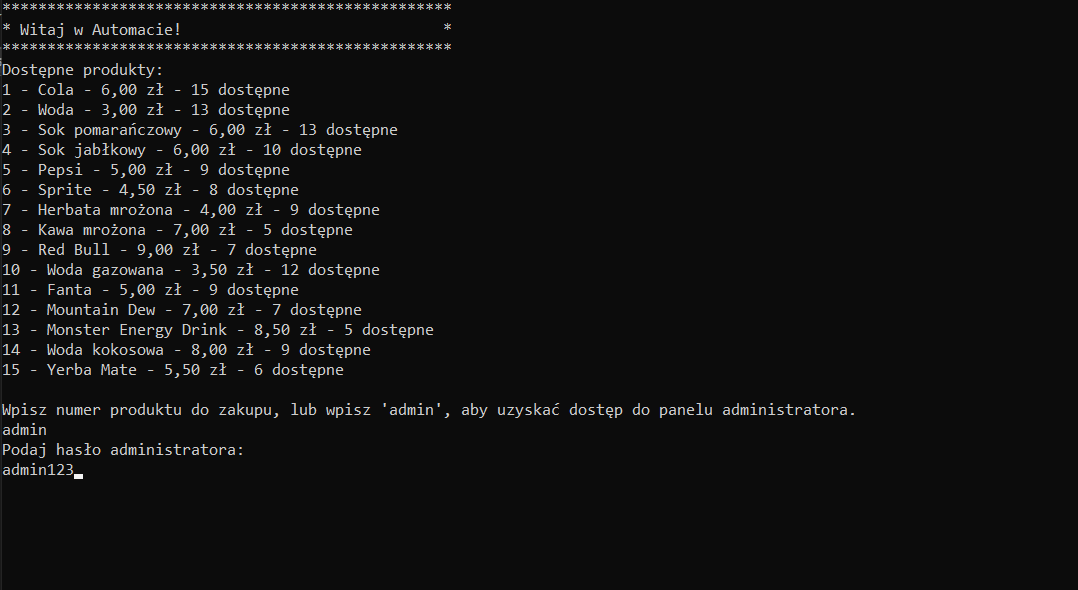
\includegraphics[width=0.8\textwidth]{grafiki/admin_log.png}
    \caption{\footnotesize Admin - logowanie}	
    \label{fig:5.2}

\end{figure}

Na rys. \ref{fig:5.2} Logowanie do panelu admina za pomocą hasła 

\begin{figure}[H] 
    \centering
    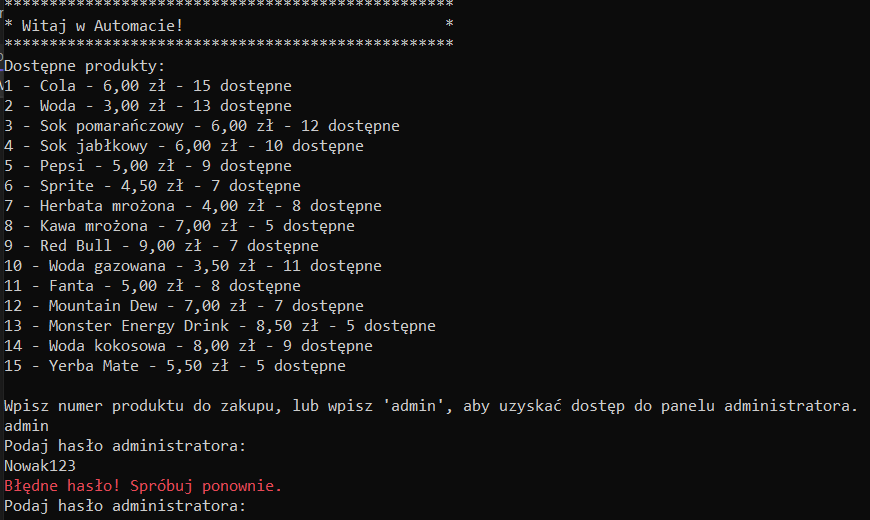
\includegraphics[width=0.8\textwidth]{grafiki/blad_admin_haslo1.png}
    \caption{\footnotesize Admin - logowanie błąd}	
    \label{fig:5.3}

\end{figure}

Na rys. \ref{fig:5.3} Widać błąd ponieważ hasło które zostało podane jest niepoprawne.

\newpage

\begin{figure}[H] 
    \centering
    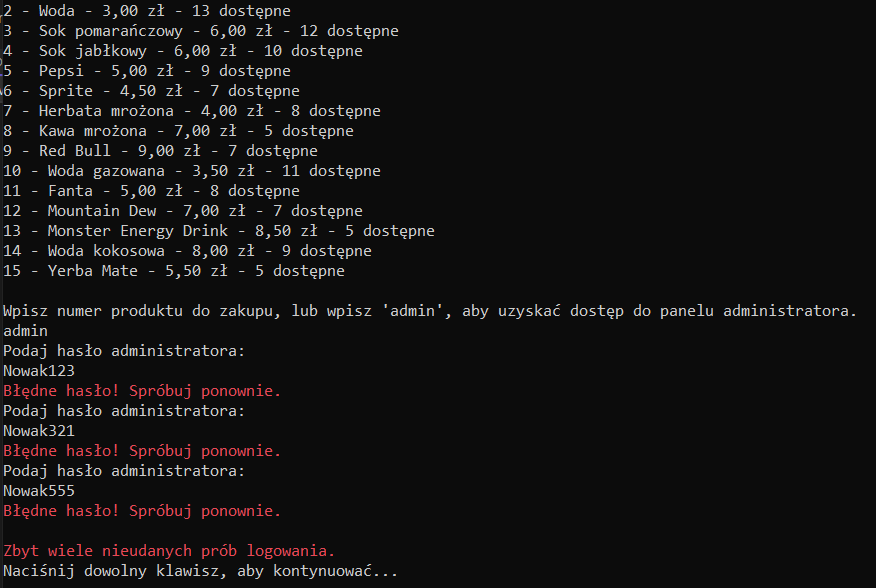
\includegraphics[width=0.8\textwidth]{grafiki/blad_admin_haslo2.png}
    \caption{\footnotesize Admin - logowanie 3 nieudane próby}	
    \label{fig:5.4}

\end{figure}

Na rys. \ref{fig:5.4} Gdy wprowadzone hasło będzie nieprawidłowe trzykrotnie wyświetli się komunikat o zbyt wielu nieudanych próbach logowania.

% ********************

\section{Zakup produktu}

 \begin{figure}[H] 
    \centering
    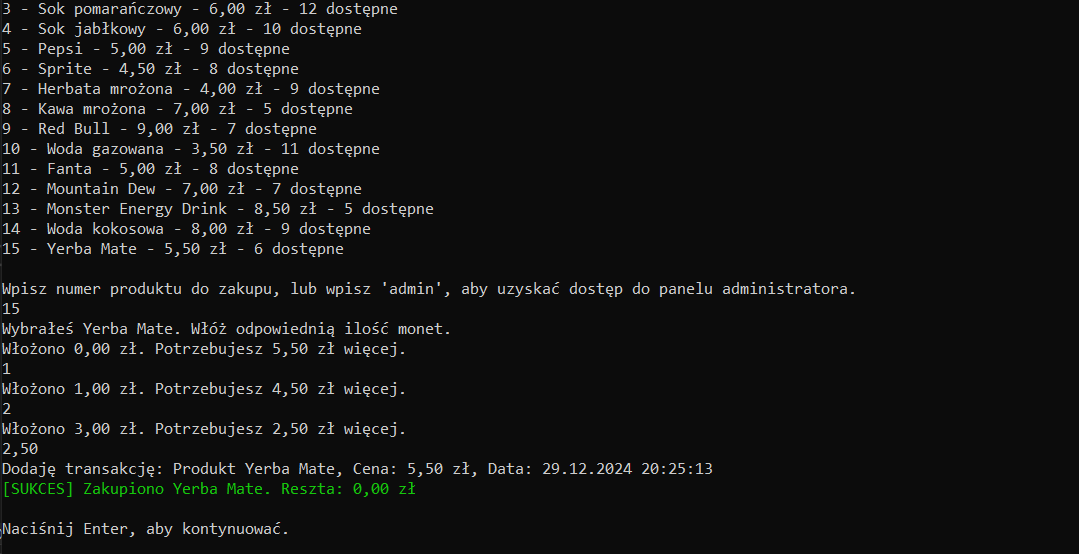
\includegraphics[width=0.8\textwidth]{grafiki/zakup_produktu_bez_reszty.png}
    \caption{\footnotesize Zakup produktu:}	
    \label{fig:5.5}
\end{figure}



Pozwala klientowi na prosty zakup produktu z listy a jeśli trzeba wydaje jego resztę.


\begin{figure}[H] 
    \centering
    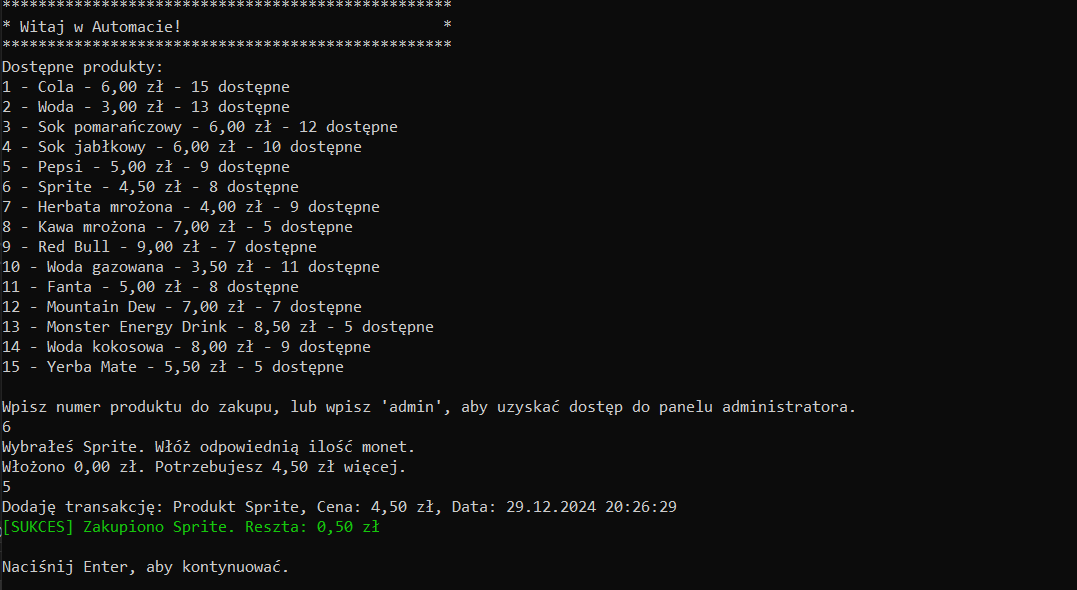
\includegraphics[width=0.8\textwidth]{grafiki/zakup_produktu_reszta.png}
    \caption{\footnotesize Zakup produktu - wydanie reszty dla klienta}	
    \label{fig:5.6}
\end{figure}

Jak widać podczas zakupu automat prosi klienta o podaną kwotę którą może wpłacać na raty a w razie potrzeby wydaje mu jego resztę oraz wyświetla się komunikat o sukcesie dokonania zakupu.



\begin{figure}[H] 
    \centering
    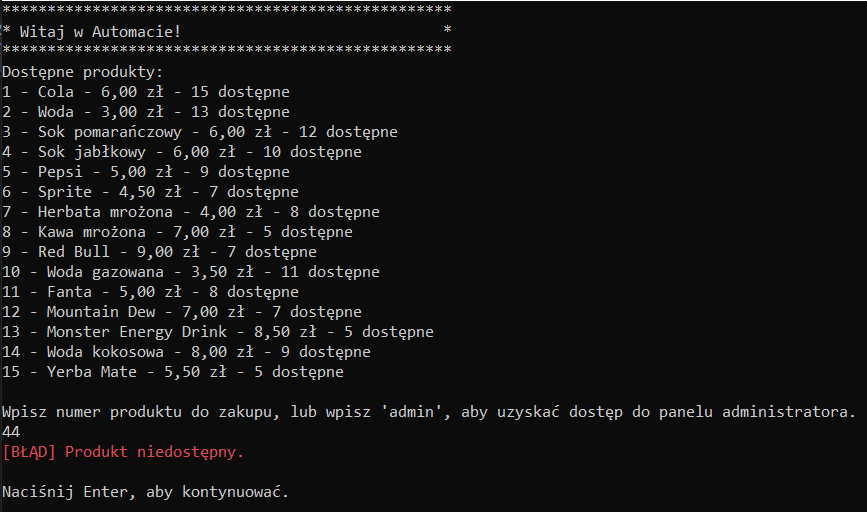
\includegraphics[width=0.8\textwidth]{grafiki/blad_zakupu.png}
    \caption{\footnotesize Zakup produktu - błędne ID}	
    \label{fig:5.7}
\end{figure}

Gdy wypiszemy błędne ID podczas zakupu dostaniemy informacje że produkt nie jest dostępny.


\newpage

 
\section{Menu admina}

Jest to menu, które umożliwia adminowi na dodawanie usuwanie oraz edytowanie produktów. Może on także wyświetlić listę transakcji, sprawdzić ile pieniędzy aktualnie znajduje się w automacie, wpłacić lub wypłacić pieniądze z automatu.

\begin{figure}[H] 
    \centering
    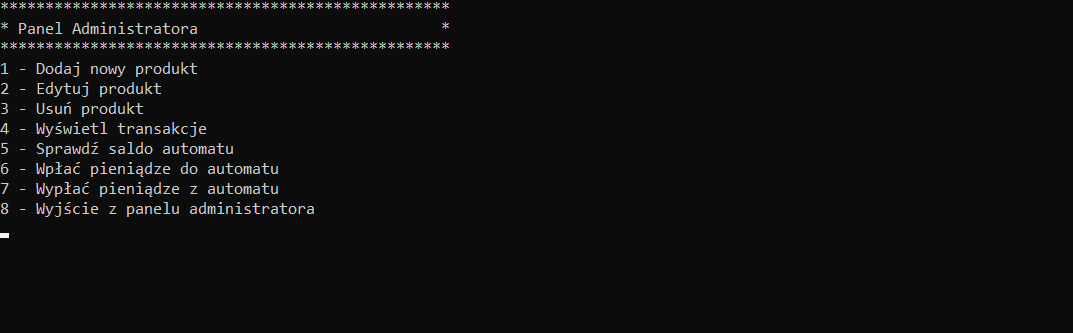
\includegraphics[width=0.8\textwidth]{grafiki/menu_admin.png}
    \caption{\footnotesize Menu admina}	
    \label{fig:5.8}
\end{figure}

W menu admina mamy do wyboru osiem opcji takich jak: dodanie nowego produktu, edycja produktu, usunięcie produktu, wyświetlenie transakcji, sprawdzenie salda, wpłacenie pieniędzy do automatu, wypłacenie pieniędzy z automatu oraz wyjście.



\begin{figure}[H] 
    \centering
    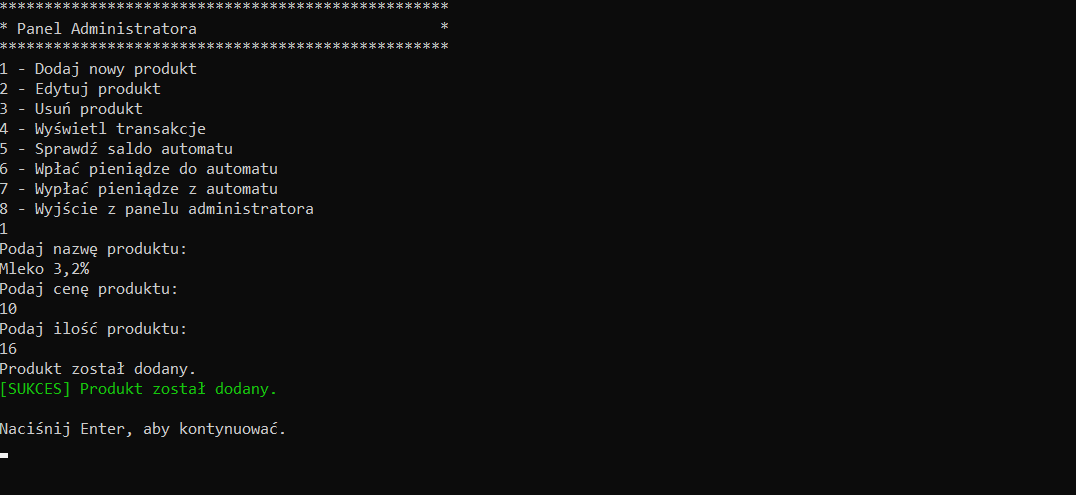
\includegraphics[width=0.8\textwidth]{grafiki/dodanie_produktu.png}
    \caption{\footnotesize Menu admina - dodanie produktu}	
    \label{fig:5.9}
\end{figure}
Aby dodać nowy produkt do automatu, konieczne jest podanie jego nazwy, ceny oraz dostępnej ilości. Każdy z tych parametrów jest niezbędny, aby produkt mógł zostać prawidłowo zapisany w systemie i udostępniony klientom.


\newpage


\begin{figure}[H] 
    \centering
    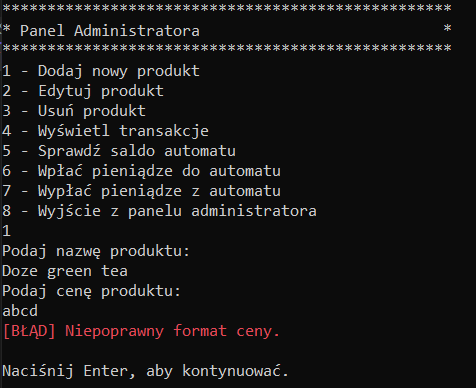
\includegraphics[width=0.8\textwidth]{grafiki/blad_format_ceny.png}
    \caption{\footnotesize Menu admina - dodanie produktu błąd formatu ceny}	
    \label{fig:5.10}
\end{figure}
Podczas wprowadzania ceny produktu należy upewnić się, że jej format jest prawidłowy. Cena powinna być zapisana jako wartość liczbowa z separatorami dziesiętnymi zgodnymi z przyjętym standardem. Nieprawidłowy format może uniemożliwić dodanie produktu lub prowadzić do błędów w działaniu systemu.

\newpage


\begin{figure}[H] 
    \centering
    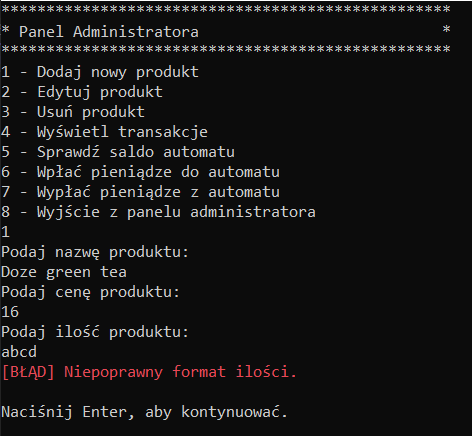
\includegraphics[width=0.8\textwidth]{grafiki/blad_format_ilosci.png}
    \caption{\footnotesize Menu admina - dodanie produktu błąd format ilości}	
    \label{fig:5.11}
\end{figure}
Przed zapisaniem nowego produktu w bazie danych należy sprawdzić, czy podana ilość jest poprawna. System akceptuje wyłącznie wartości liczbowe, które określają liczbę dostępnych sztuk danego produktu w automacie. Wprowadzenie błędnego formatu może skutkować nieprawidłowym działaniem aplikacji.

\newpage


\begin{figure}[H] 
    \centering
    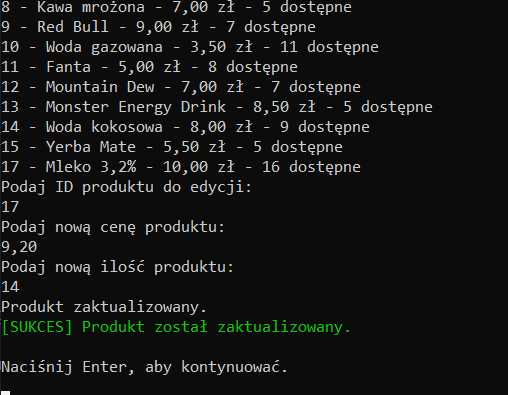
\includegraphics[width=0.8\textwidth]{grafiki/edycja_produktu.png}
    \caption{\footnotesize Menu admina - edycja produktu}	
    \label{fig:5.12}
\end{figure}
Jeśli chcemy edytować dane produktu, musimy najpierw wybrać jego unikalny identyfikator (ID). Następnie podajemy nową cenę oraz ilość, która ma zostać zaktualizowana w systemie. Warto pamiętać, aby upewnić się, że wprowadzane wartości są poprawne, ponieważ błędne dane mogą wpłynąć na dostępność i wycenę produktu w automacie.

\newpage

\begin{figure}[H] 
    \centering
    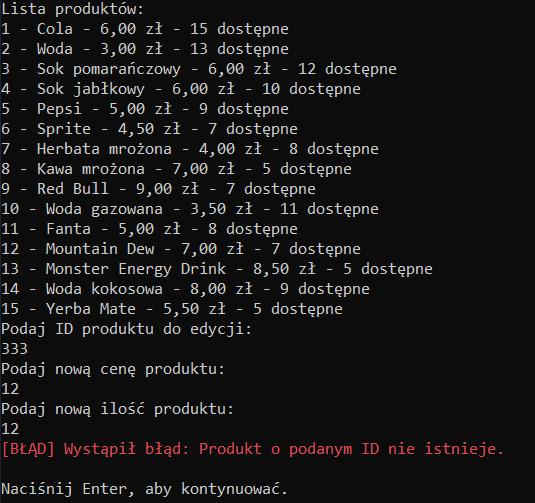
\includegraphics[width=0.8\textwidth]{grafiki/blad_id_edycja.png}
    \caption{\footnotesize Menu admina - edycja produktu błędne ID}	
    \label{fig:5.13}
\end{figure}
Na rys. \ref{fig:5.13} Podczas próby edycji produktu możemy zauważyć błąd wynikający z podania nieprawidłowego identyfikatora (ID). Oznacza to, że w systemie nie istnieje produkt o wskazanym ID, co uniemożliwia jego modyfikację.

\newpage

\begin{figure}[H] 
    \centering
    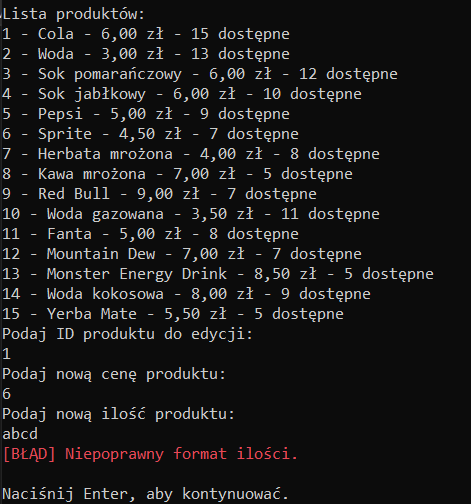
\includegraphics[width=0.8\textwidth]{grafiki/blad_ilosc_edycja.png}
    \caption{\footnotesize Menu admina - edycja produktu zły format ilości}	
    \label{fig:5.14}
\end{figure}
Na rys. \ref{fig:5.14} System zgłasza błąd, ponieważ podany format ilości produktu podczas edycji jest nieprawidłowy. Wartość ta powinna być liczbą całkowitą, oznaczającą dostępny stan magazynowy produktu w automacie. Niepoprawny format może skutkować błędnym działaniem systemu.

\newpage


\begin{figure}[H] 
    \centering
    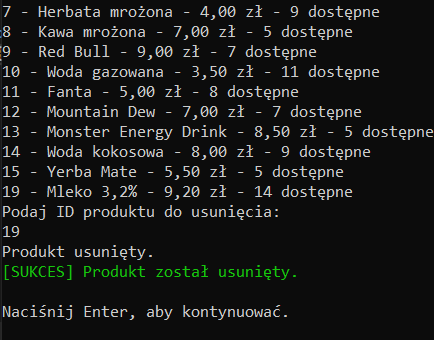
\includegraphics[width=0.8\textwidth]{grafiki/usun_produkt.png}
    \caption{\footnotesize Menu admina - usuwanie produktu}	
    \label{fig:5.15}
\end{figure}

Aby usunąć wybrany produkt z systemu, należy skorzystać z opcji "3 - Usuń produkt" w menu administratora. Następnie wymagane jest podanie poprawnego identyfikatora (ID) produktu znajdującego się na liście. Po potwierdzeniu operacji produkt zostanie usunięty z bazy danych.

\newpage

\begin{figure}[H] 
    \centering
    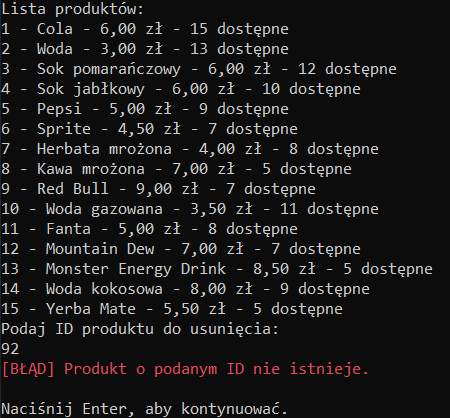
\includegraphics[width=0.8\textwidth]{grafiki/blad_id_usun.png}
    \caption{\footnotesize Menu admina - usuwanie produktu błąd}	
    \label{fig:5.16}
\end{figure}

Na rys. \ref{fig:5.16} W przypadku podania nieprawidłowego identyfikatora (ID) system nie pozwoli na usunięcie produktu. Jeśli dany ID nie istnieje w bazie, operacja zostanie przerwana, a użytkownik otrzyma stosowny komunikat o błędzie.

\newpage

\begin{figure}[H] 
    \centering
    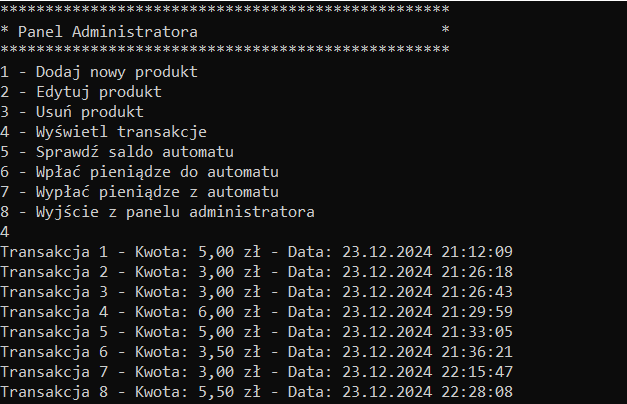
\includegraphics[width=0.8\textwidth]{grafiki/wyswietl_transakcje.png}
    \caption{\footnotesize Menu admina - wyświetl transakcje}	
    \label{fig:5.17}
\end{figure}

Po wybraniu opcji "4 - Wyświetl transakcje" uzyskujemy dostęp do historii dokonanych transakcji w automacie z napojami. Dzięki temu administrator może przeanalizować wcześniejsze zakupy użytkowników.

\begin{figure}[H] 
    \centering
    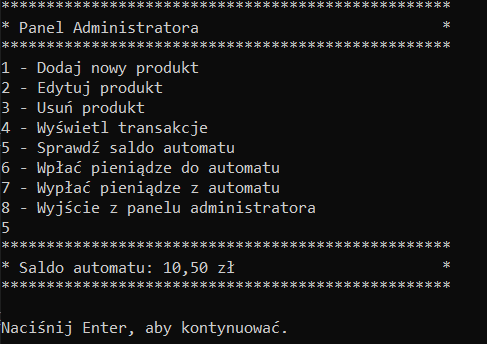
\includegraphics[width=0.8\textwidth]{grafiki/saldo_automatu.png}
    \caption{\footnotesize Menu admina - saldo automatu}	
    \label{fig:5.18}
\end{figure}

Aplikacja pozwala też na sprawdzenie salda automatu.

\newpage

\begin{figure}[H] 
    \centering
    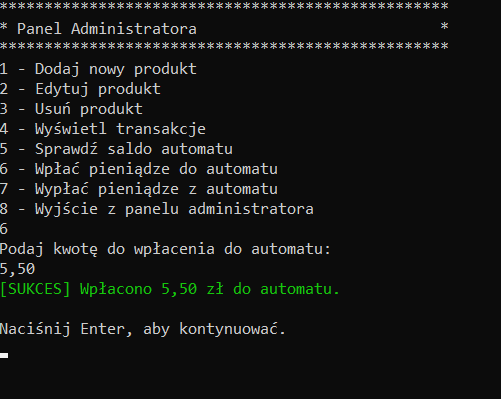
\includegraphics[width=0.8\textwidth]{grafiki/wplacanie_automat.png}
    \caption{\footnotesize Menu admina - dodawanie salda automatu}	
    \label{fig:5.19}
\end{figure}

Gdy automat jest pusty możemy wpłacić pieniądze żeby maszyna mogła wydawać resztę.

\begin{figure}[H] 
    \centering
    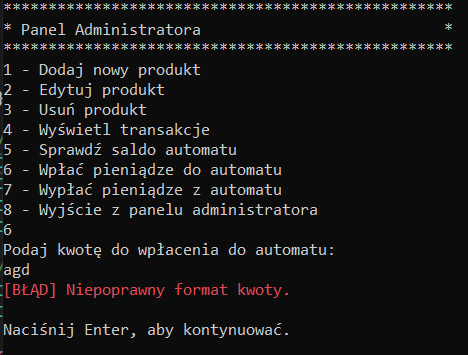
\includegraphics[width=0.8\textwidth]{grafiki/blad_wplata.png}
    \caption{\footnotesize Menu admina - dodawanie salda automatu}	
    \label{fig:5.20}
\end{figure}

Na rys. \ref{fig:5.20} Podczas wpłacania pieniędzy do automatu należy upewnić się, że wprowadzony format kwoty jest poprawny. W przeciwnym razie system wyświetli błąd.

\begin{figure}[H] 
    \centering
    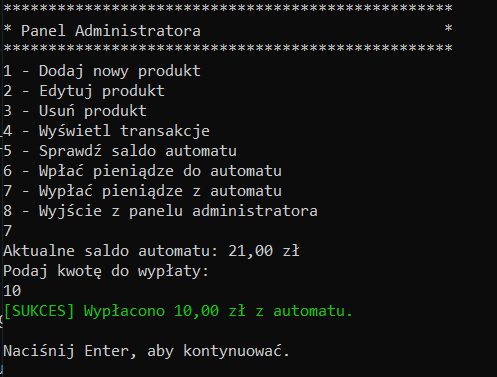
\includegraphics[width=0.8\textwidth]{grafiki/wyplacanie_pieniedzy.png}
    \caption{\footnotesize Menu admina - wyciąganie pieniędzy z automatu}	
    \label{fig:5.21}
\end{figure}

Aplikacja posiada też funkcję wypłaty pieniędzy z automatu.

\begin{figure}[H] 
    \centering
    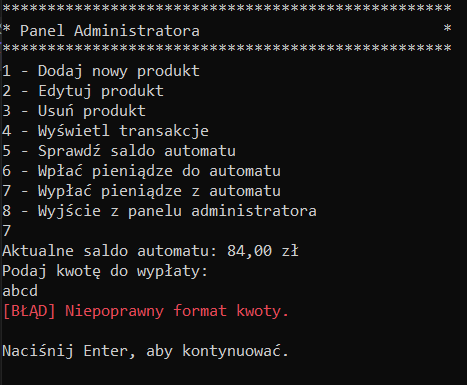
\includegraphics[width=0.8\textwidth]{grafiki/blad_format_wyplac.png}
    \caption{\footnotesize Menu admina - wyciąganie pieniędzy z automatu błąd formatu}	
    \label{fig:5.22}
\end{figure}

Aplikacja sprawdza czy format kwoty podczas wypłaty jest poprawny.

\begin{figure}[H] 
    \centering
    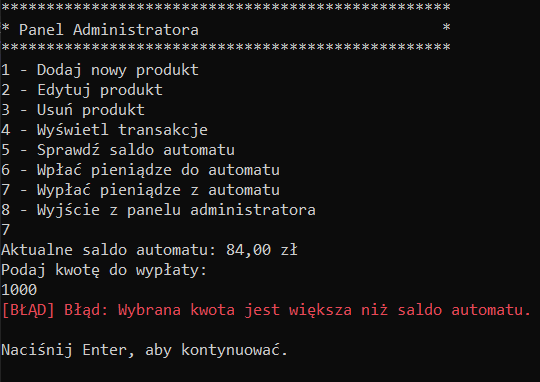
\includegraphics[width=0.8\textwidth]{grafiki/blad_kwota_wyplac.png}
    \caption{\footnotesize Menu admina - wyciąganie pieniędzy z automatu błąd formatu}	
    \label{fig:5.23}
\end{figure}

Jeśli kwota którą chcemy wyciągnąć jest większa niż saldo automatu to wystąpi błąd.



\chapter{Podsumowanie}

\section{Podsumowanie}
Aplikacja automatu z napojami oferuje kompleksowe rozwiązania umożliwiające zarządzanie produktami, transakcjami, stanem automatu oraz obsługą błędów. Główne menu zapewnia łatwy wybór i zakup produktu. Panel administratora pozwala na rzeczy takie jak dodawanie, edytowanie oraz usuwanie produktu. Pozwala nam także na przeglądanie historii transakcji, zarządzanie saldem automatu oraz wyjście z aplikacji. Logowanie zapewnia bezpieczny dostęp do systemu, a admin może efektywnie zarządzać automatem. Dzięki tym funkcjom aplikacja pozwala na poprawę obsługi klienta oraz optymalizację operacji związanych z zarządzaniem maszyną.

\section{Dalszy rozwój projektu}

Projekt automatu z napojami może być rozbudowywany w różnych kierunkach, aby zwiększyć jego funkcjonalność i użyteczność. Jednym z możliwych kierunków jest zwiększenie poziomu bezpieczeństwa aplikacji, np. poprzez dodanie bardziej zaawansowanych mechanizmów autentykacji lub szyfrowania danych użytkowników.

Dodatkowo, warto rozważyć implementację funkcji importowania i eksportowania danych z plików XLS lub CSV, co umożliwiłoby łatwe zarządzanie danymi, takimi jak zapasy produktów, transakcje czy raporty o stanie maszyny. Taka funkcjonalność pozwoliłaby na lepszą integrację aplikacji z systemami zewnętrznymi i ułatwiłaby obsługę dużych zbiorów danych.

Kolejnym obszarem rozwoju może być dodanie mechanizmu promocji, który umożliwiłby użytkownikom korzystanie z różnych ofert rabatowych lub zniżek na produkty. Może to zwiększyć zaangażowanie klientów i poprawić wyniki sprzedaży.

Warto również rozważyć integrację z nowoczesnymi metodami płatności, takimi jak portfele cyfrowe, płatności mobilne czy karty lojalnościowe, co poprawiłoby wygodę korzystania z automatu i zapewniłoby większą elastyczność w dokonywaniu płatności.
% ********** Koniec rozdziału **********